\documentclass[12pt,a4paper]{article}
\usepackage{amsmath,amsthm,amssymb,mathtools}
\usepackage{tikz}
\usetikzlibrary{arrows.meta,positioning,shapes.geometric,calc,fit,backgrounds}
\usepackage{graphicx}
\usepackage{booktabs,tabularx,multirow}
\usepackage[ruled,vlined,linesnumbered]{algorithm2e}
\usepackage[most]{tcolorbox}
\usepackage{hyperref}
\usepackage[capitalize,noabbrev]{cleveref}
\usepackage[margin=1in]{geometry}
\usepackage{fancyhdr}
\usepackage{enumitem}
\usepackage{xcolor}

%% ── tcolorbox environments ──────────────────────────────────────────────────
\newtcolorbox{keyinsight}[1][]{colback=blue!5!white,colframe=blue!75!black,
  fonttitle=\bfseries,title=Key Insight,#1}
\newtcolorbox{example}[1][]{colback=green!5!white,colframe=green!75!black,
  fonttitle=\bfseries,title=Example,#1}
\newtcolorbox{warningbox}[1][]{colback=red!5!white,colframe=red!75!black,
  fonttitle=\bfseries,title=Warning,#1}

%% ── amsthm environments ─────────────────────────────────────────────────────
\newtheorem{theorem}{Theorem}[section]
\newtheorem{lemma}[theorem]{Lemma}
\newtheorem{definition}{Definition}[section]
\newtheorem{remark}{Remark}[section]

%% ── Page style ───────────────────────────────────────────────────────────────
\pagestyle{fancy}
\fancyhf{}
\rhead{Deep Learning -- Session 15}
\lhead{CNN Parameter Calculations \& L2 Regularisation}
\cfoot{\thepage}
\renewcommand{\headrulewidth}{0.4pt}

%% ── Hyperref colours ─────────────────────────────────────────────────────────
\hypersetup{
  colorlinks=true,
  linkcolor=blue!60!black,
  citecolor=green!50!black,
  urlcolor=blue!70!black
}

%% ── Convenience macros ───────────────────────────────────────────────────────
\newcommand{\Cin}{C_{\mathrm{in}}}
\newcommand{\Cout}{C_{\mathrm{out}}}
\newcommand{\Ltotal}{\mathcal{L}_{\mathrm{total}}}
\newcommand{\Ldata}{\mathcal{L}_{\mathrm{data}}}
\newcommand{\floor}[1]{\left\lfloor #1 \right\rfloor}

% ─────────────────────────────────────────────────────────────────────────────
\begin{document}

% ════════════════════════════════════════════════════════════════════════════
%  TITLE PAGE
% ════════════════════════════════════════════════════════════════════════════
\begin{titlepage}
  \centering
  \vspace*{2cm}
  {\LARGE\bfseries Deep Learning with PyTorch\\[0.4em]
   \large IIIT Dharwad --- Course Lecture Notes\par}
  \vspace{1.5cm}
  \rule{\linewidth}{0.5pt}\\[0.4em]
  {\huge\bfseries Session 15\\[0.3em]
   \Large CNN Parameter Calculations,\\
   Output Size Formulae, and\\
   L2 Regularisation\par}
  \rule{\linewidth}{0.5pt}
  \vspace{1.5cm}
  \begin{tabular}{ll}
    \textbf{Session Number:} & 15 \\[4pt]
    \textbf{Topic:}          & CNN Exam Q\&A --- Parameter Counting, \\
                             & Convolution Output Sizes, L2 Regularisation \\[4pt]
    \textbf{Slide Deck:}     & \texttt{08\_PyTorchDL\_RNN} (transition deck) \\[4pt]
    \textbf{Instructors:}    & Prof.\ S.~R.~M.\ Prasanna \&
                               Dr.\ Sunil Saumya \\[4pt]
    \textbf{Institution:}    & IIIT Dharwad \\[4pt]
    \textbf{Date:}           & Academic Year 2024--25 \\[4pt]
    \textbf{Video:}          & \url{https://vimeo.com/1153110691} \\
  \end{tabular}
  \vfill
  {\small These notes are compiled from the session transcript and visual
   extractions. Session 15 was conducted as a student-driven Q\&A and
   doubt-clearing session covering CNN parameter calculations, convolution
   output size formulae, and L2 regularisation, serving as consolidation
   before the transition to Recurrent Neural Networks.}
\end{titlepage}

% ════════════════════════════════════════════════════════════════════════════
%  TABLE OF CONTENTS
% ════════════════════════════════════════════════════════════════════════════
\tableofcontents
\newpage

% ════════════════════════════════════════════════════════════════════════════
\section{Introduction}
\label{sec:intro}
% ════════════════════════════════════════════════════════════════════════════

Session 15 of the \emph{Deep Learning with PyTorch} course at IIIT Dharwad
was conducted as an interactive Q\&A and doubt-clearing class rather than a
conventional lecture. No slide deck was screen-shared; instead, students
raised questions on camera and the instructors---Prof.\ S.~R.~M.\ Prasanna
and Dr.\ Sunil Saumya---clarified key concepts from the preceding CNN
sessions in real time.

The session centred on three tightly connected topics:

\begin{enumerate}[label=\textbf{(\arabic*)}]
  \item \textbf{Convolutional layer parameter counting}: How to derive the
        exact number of trainable weights and biases in a single
        \texttt{Conv2d} layer, and why the count is dramatically smaller
        than an equivalent fully-connected layer.
  \item \textbf{Output spatial size with padding}: The general formula
        $\floor{(N - F + 2P)/S} + 1$ and the three most common padding
        regimes encountered in practice.
  \item \textbf{L2 regularisation (weight decay)}: The relationship between
        the mathematical penalty $\lambda \sum_i w_i^2$, the gradient update
        rule, and PyTorch's \texttt{weight\_decay} argument in
        \texttt{optim.Adam} and \texttt{optim.SGD}.
\end{enumerate}

Together, these topics represent core ``nuts and bolts'' knowledge that
every practitioner must be comfortable with before moving to more complex
architectures. \Cref{sec:background} reviews the CNN building blocks
required as prerequisites. \Cref{sec:param_count} treats parameter counting
in depth. \Cref{sec:output_size} covers output size formulae.
\Cref{sec:l2reg} develops L2 regularisation theory and its PyTorch
implementation. \Cref{sec:comparison} places these ideas in a broader
comparative context. \Cref{sec:conclusion} summarises the session and
previews the transition to Recurrent Neural Networks.

\begin{keyinsight}
This session bridges the CNN module and the forthcoming RNN module. Mastery
of parameter counting and regularisation is prerequisite for reasoning about
model capacity, computational cost, and generalisation in any architecture.
\end{keyinsight}

% ════════════════════════════════════════════════════════════════════════════
\section{Background and Prerequisites}
\label{sec:background}
% ════════════════════════════════════════════════════════════════════════════

\subsection{Convolutional Neural Network Recap}

A Convolutional Neural Network (CNN) processes grid-structured data (images,
feature maps) through a sequence of learnable linear filters followed by
non-linear activations and spatial pooling. The key inductive biases
exploited are \emph{local connectivity} and \emph{weight sharing}.

\begin{definition}[Convolutional Layer]
\label{def:conv_layer}
A convolutional layer with $\Cout$ filters, each of spatial size $F \times F$
applied to an input tensor of spatial size $N \times N$ with $\Cin$ channels
produces an output tensor of shape
\[
  \Cout \;\times\;
  \underbrace{\floor{\tfrac{N - F + 2P}{S}} + 1}_{H_{\mathrm{out}}}
  \;\times\;
  \underbrace{\floor{\tfrac{N - F + 2P}{S}} + 1}_{W_{\mathrm{out}}}
\]
where $P$ is zero-padding (per side) and $S$ is the stride.
\end{definition}

\subsection{Notation Summary}

\Cref{tab:notation} collects the symbols used throughout these notes.

\begin{table}[ht]
  \centering
  \caption{Notation used in Session 15 notes.}
  \label{tab:notation}
  \begin{tabular}{@{}cll@{}}
    \toprule
    Symbol & Meaning & Typical values \\
    \midrule
    $N$     & Input spatial dimension (height or width) & 7, 28, 224 \\
    $F$     & Filter/kernel spatial size                & 1, 3, 5    \\
    $\Cin$  & Number of input channels                  & 1, 3, 64, 128 \\
    $\Cout$ & Number of output filters                  & 32, 64, 256 \\
    $P$     & Zero-padding (applied each side)          & 0, 1, 2 \\
    $S$     & Stride                                    & 1, 2 \\
    $\lambda$ & L2 regularisation coefficient           & $10^{-4}$--$10^{-2}$ \\
    $\eta$  & Learning rate                             & $10^{-3}$--$10^{-1}$ \\
    \bottomrule
  \end{tabular}
\end{table}

\subsection{PyTorch \texttt{Conv2d} API}

In PyTorch the primary interface is:

\begin{verbatim}
torch.nn.Conv2d(in_channels, out_channels, kernel_size,
                stride=1, padding=0, bias=True)
\end{verbatim}

The argument \texttt{bias=True} (default) adds one learnable scalar bias per
output filter. This single flag controls whether bias terms appear in the
parameter count.

\begin{remark}
\label{rem:bias_default}
Because \texttt{bias=True} is the default, exam questions that do not
explicitly state ``no bias'' should be answered \emph{with} bias terms
included. During the session, the instructors confirmed this interpretation.
\end{remark}

% ════════════════════════════════════════════════════════════════════════════
\section{Convolutional Layer Parameter Counting}
\label{sec:param_count}
% ════════════════════════════════════════════════════════════════════════════

\subsection{Derivation of the Parameter Formula}

Each output filter is a 3-D weight tensor of shape $F \times F \times \Cin$
plus one scalar bias. There are $\Cout$ such filters. The total number of
trainable parameters is therefore

\begin{equation}
  \label{eq:param_formula}
  \boxed{P_{\mathrm{conv}} = \bigl(F \times F \times \Cin + 1\bigr) \times \Cout}
\end{equation}

\noindent
where the $+1$ accounts for the bias term. If \texttt{bias=False} is set,
the formula reduces to $(F^2 \cdot \Cin) \cdot \Cout$.

\begin{keyinsight}
The parameter count of a \texttt{Conv2d} layer is \emph{independent of the
input spatial size} $N$. Doubling the input resolution does \emph{not} change
the number of learnable parameters---it only changes the number of times each
filter is applied (the number of output locations). This is the essence of
\textbf{weight sharing}.
\end{keyinsight}

\subsection{Worked Example: 64 Filters, 3\texttimes3, 128 Input Channels}

The exam question that arose during Session 15 was:

\begin{quote}
\itshape
``A convolutional layer has 64 filters, a kernel size of $3 \times 3$, and
128 input channels. How many trainable parameters does it have?''
\end{quote}

Applying \cref{eq:param_formula} with $F = 3$, $\Cin = 128$, $\Cout = 64$:

\begin{align}
  P_{\mathrm{conv}}
    &= \bigl(3 \times 3 \times 128 + 1\bigr) \times 64 \notag \\
    &= \bigl(1152 + 1\bigr) \times 64 \notag \\
    &= 1153 \times 64 \notag \\
    &= \mathbf{73{,}792} \label{eq:example_count}
\end{align}

\noindent
\textbf{Breakdown:}
\begin{itemize}[noitemsep]
  \item Weight parameters: $3 \times 3 \times 128 \times 64 = 73{,}728$
  \item Bias parameters: $64$ (one per output filter)
  \item \textbf{Total: $73{,}792$}
\end{itemize}

\begin{example}[title=Step-by-step parameter count]
\textbf{Given:} \texttt{nn.Conv2d(128, 64, kernel\_size=3)}

\medskip
\begin{tabular}{@{}lrl@{}}
  \toprule
  Component & Calculation & Value \\
  \midrule
  Weights per filter & $3 \times 3 \times 128$ & 1,152 \\
  Filters            & 64                      & --- \\
  Total weights      & $1152 \times 64$        & 73,728 \\
  Bias terms         & $1 \times 64$           & 64 \\
  \midrule
  \textbf{Grand total} & $73728 + 64$ & \textbf{73,792} \\
  \bottomrule
\end{tabular}
\end{example}

\subsection{Parameter Counting TikZ Diagram}
\label{subsec:param_diagram}

\Cref{fig:param_count} illustrates the weight-sharing structure that leads
to \cref{eq:param_formula}.

\begin{figure}[ht]
\centering
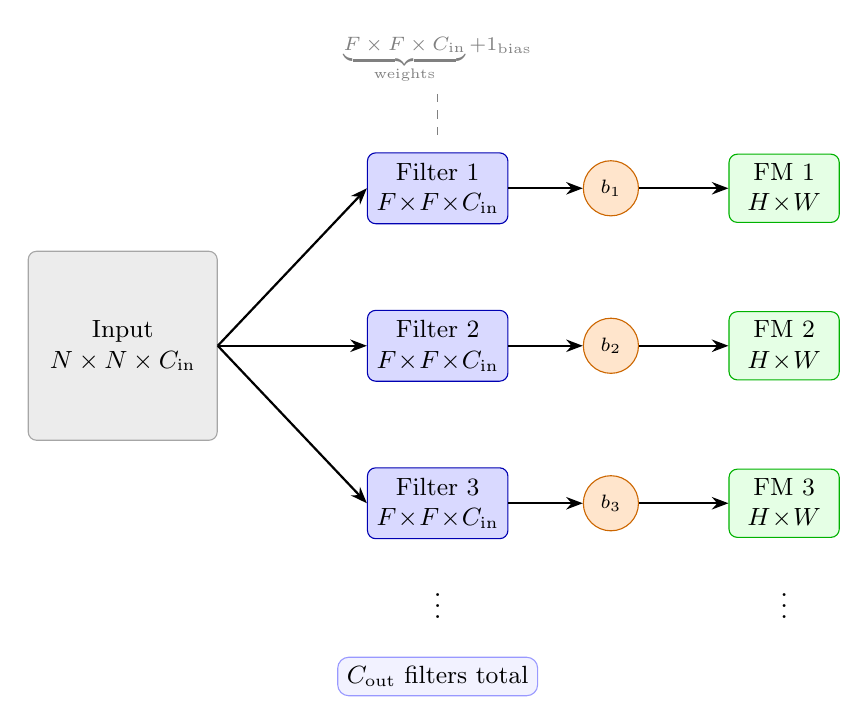
\begin{tikzpicture}[
  filter/.style={draw=blue!70!black, fill=blue!15, rounded corners=3pt,
                 minimum width=1.6cm, minimum height=0.9cm, font=\small},
  input/.style={draw=gray!70, fill=gray!15, rounded corners=3pt,
                minimum width=2.4cm, minimum height=2.4cm, font=\small},
  bias/.style={draw=orange!80!black, fill=orange!20, circle,
               minimum size=0.7cm, font=\scriptsize},
  arrow/.style={-{Stealth[length=6pt]}, thick},
  every node/.style={align=center}
]

%% Input volume
\node[input] (inp) at (0,0) {Input\\$N\times N\times\Cin$};

%% Three representative filters
\foreach \i/\y in {1/2.0, 2/0, 3/-2.0}{
  \node[filter] (f\i) at (4.0,\y) {Filter $\i$\\$F\!\times\!F\!\times\!\Cin$};
  \node[bias]   (b\i) at (6.2,\y) {$b_\i$};
  \draw[arrow] (inp.east) -- (f\i.west);
  \draw[arrow] (f\i.east) -- (b\i.west);
}

%% Output feature maps
\foreach \i/\y in {1/2.0, 2/0, 3/-2.0}{
  \node[draw=green!70!black, fill=green!10, rounded corners=3pt,
        minimum width=1.4cm, minimum height=0.8cm, font=\small]
        (o\i) at (8.4,\y) {FM $\i$\\$H\!\times\!W$};
  \draw[arrow] (b\i.east) -- (o\i.west);
}

%% Ellipsis
\node at (4.0,-3.2) {$\vdots$};
\node at (8.4,-3.2) {$\vdots$};

%% Label: Cout filters total
\node[draw=blue!40, fill=blue!5, rounded corners=4pt,
      font=\small, minimum width=2.0cm]
     at (4.0,-4.2) {$\Cout$ filters total};

%% Annotation arrows
\draw[dashed, gray] (4.0, 3.2) -- (4.0, 2.6)
  node[above, font=\scriptsize, at start]
  {$\underbrace{F\times F\times\Cin}_{\text{weights}} + 1_{\text{bias}}$};

\end{tikzpicture}
\caption{Weight-sharing in a convolutional layer. Each of the $\Cout$ filters
  has $F \times F \times \Cin$ weight parameters and one bias, giving
  $(F^2 \Cin + 1)\Cout$ total parameters. All output locations share the same
  filter weights.}
\label{fig:param_count}
\end{figure}

\subsection{Algorithm: Computing Parameters Programmatically}

\Cref{alg:param_count} provides a systematic procedure for counting
parameters across a full CNN.

\begin{algorithm}[ht]
\DontPrintSemicolon
\caption{Count Trainable Parameters in a CNN}
\label{alg:param_count}
\KwIn{CNN model with layers $\ell = 1, \ldots, L$}
\KwOut{Total parameter count $P_{\mathrm{total}}$}

$P_{\mathrm{total}} \leftarrow 0$\;
\For{each layer $\ell$ in model}{
  \uIf{$\ell$ is \texttt{Conv2d}($\Cin$, $\Cout$, $F$, \texttt{bias}$=b$)}{
    $P_\ell \leftarrow F \times F \times \Cin \times \Cout$\;
    \If{$b = \mathrm{True}$}{
      $P_\ell \leftarrow P_\ell + \Cout$
        \tcp*{one bias per output filter}
    }
  }
  \uElseIf{$\ell$ is \texttt{Linear}($d_{\mathrm{in}}$, $d_{\mathrm{out}}$, \texttt{bias}$=b$)}{
    $P_\ell \leftarrow d_{\mathrm{in}} \times d_{\mathrm{out}}$\;
    \If{$b = \mathrm{True}$}{
      $P_\ell \leftarrow P_\ell + d_{\mathrm{out}}$
    }
  }
  \uElseIf{$\ell$ is \texttt{BatchNorm2d}($C$)}{
    $P_\ell \leftarrow 2C$
      \tcp*{scale $\gamma$ and shift $\beta$, one per channel}
  }
  \Else{
    $P_\ell \leftarrow 0$
      \tcp*{Activation, Pooling, Dropout have no parameters}
  }
  $P_{\mathrm{total}} \leftarrow P_{\mathrm{total}} + P_\ell$\;
}
\Return $P_{\mathrm{total}}$\;
\end{algorithm}

\subsection{Comparison: Conv2d vs Fully-Connected Layer}

A critical insight from the session is that weight sharing makes CNNs
dramatically more parameter-efficient than fully-connected (FC) layers for
the same representational task.

\begin{keyinsight}
For a 128-channel $7 \times 7$ feature map fed into 64 units:
\begin{align*}
  P_{\mathrm{conv}} &= (3 \times 3 \times 128 + 1) \times 64 = 73{,}792 \\
  P_{\mathrm{FC}}   &= (7 \times 7 \times 128 + 1) \times 64
                     = (6272 + 1) \times 64 = 401{,}472
\end{align*}
The convolutional layer uses roughly $\mathbf{5.4\times}$ fewer parameters
while scanning the entire $7 \times 7$ spatial grid.
\end{keyinsight}

\begin{table}[ht]
  \centering
  \caption{Parameter comparison: \texttt{Conv2d} vs \texttt{Linear} for
    equivalent channel transformation ($\Cin=128$, $\Cout=64$).}
  \label{tab:param_comparison}
  \begin{tabularx}{\linewidth}{@{}Xrrr@{}}
    \toprule
    Layer type & Weight params & Bias params & \textbf{Total} \\
    \midrule
    \texttt{Conv2d(128,64,3)} no bias
      & $3\!\times\!3\!\times\!128\!\times\!64 = 73{,}728$  & 0 & 73,728 \\
    \texttt{Conv2d(128,64,3)} with bias
      & $73{,}728$  & 64 & \textbf{73,792} \\
    \texttt{Conv2d(128,64,5)} with bias
      & $5\!\times\!5\!\times\!128\!\times\!64 = 204{,}800$ & 64 & 204,864 \\
    \texttt{Linear(6272,64)} with bias
      & $7\!\times\!7\!\times\!128\!\times\!64 = 401{,}408$ & 64 & 401,472 \\
    \texttt{Linear(6272,64)} no bias
      & $401{,}408$ & 0 & 401,408 \\
    \bottomrule
  \end{tabularx}
\end{table}

% ════════════════════════════════════════════════════════════════════════════
\section{Convolution Output Size Formula}
\label{sec:output_size}
% ════════════════════════════════════════════════════════════════════════════

\subsection{General Formula}

The spatial dimension of the output feature map for a single axis is:

\begin{equation}
  \label{eq:output_size}
  H_{\mathrm{out}} = \floor{\frac{N - F + 2P}{S}} + 1
\end{equation}

The formula is symmetric in height and width when the input is square and
the kernel is square (which is the overwhelmingly common case). For
non-square inputs, height and width are treated independently.

\begin{definition}[Same Padding]
\label{def:same_padding}
``Same'' padding refers to the choice of $P$ such that
$H_{\mathrm{out}} = N$ when $S = 1$. Solving
\cref{eq:output_size} with $H_{\mathrm{out}} = N$ and $S = 1$:
\[
  N = \frac{N - F + 2P}{1} + 1
  \;\Longrightarrow\;
  P = \frac{F - 1}{2}
\]
This requires $F$ to be odd (the standard practice: $F \in \{1, 3, 5, 7\}$).
\end{definition}

\subsection{Common Configurations}

\Cref{tab:output_size_configs} tabulates the most common padding and stride
configurations encountered in practice.

\begin{table}[ht]
  \centering
  \caption{Output size formulae for common \texttt{Conv2d} configurations.
    Input: $N \times N$, filter $F \times F$.}
  \label{tab:output_size_configs}
  \begin{tabular}{@{}llll@{}}
    \toprule
    Configuration & Padding $P$ & Stride $S$ & Output size \\
    \midrule
    \multirow{2}{*}{No padding (``valid'')}
      & \multirow{2}{*}{0} & 1 & $N - F + 1$ \\
      &                    & 2 & $\floor{(N-F)/2}+1$ \\[4pt]
    \multirow{2}{*}{Same padding (preserve size)}
      & \multirow{2}{*}{$(F-1)/2$} & 1 & $N$ \\
      &                            & 2 & $\floor{N/2}$ \\[4pt]
    Strided (halve spatial dims) & 0 & 2 & $\floor{(N-F)/2}+1 \approx N/2$ \\
    \bottomrule
  \end{tabular}
\end{table}

\subsection{Worked Examples}

\begin{example}[title=Output sizes for a $7 \times 7$ input]
Let $N = 7$.

\medskip
\begin{tabular}{@{}llcl@{}}
  \toprule
  Layer & $(F, P, S)$ & Formula & Output \\
  \midrule
  \texttt{Conv2d(..., 3, padding=0)} & $(3,0,1)$
    & $\floor{(7-3+0)/1}+1$ & $5 \times 5$ \\
  \texttt{Conv2d(..., 3, padding=1)} & $(3,1,1)$
    & $\floor{(7-3+2)/1}+1$ & $7 \times 7$ \\
  \texttt{Conv2d(..., 3, stride=2)}  & $(3,0,2)$
    & $\floor{(7-3+0)/2}+1$ & $3 \times 3$ \\
  \texttt{Conv2d(..., 5, padding=2)} & $(5,2,1)$
    & $\floor{(7-5+4)/1}+1$ & $7 \times 7$ \\
  \bottomrule
\end{tabular}
\end{example}

\begin{example}[title=VGG-style block: $224 \to 112$]
A common pattern in VGG and similar networks uses a $3 \times 3$ conv with
same padding followed by a $2 \times 2$ max-pool with stride 2:

\begin{align*}
  \text{After conv (same)}: &\quad 224 \times 224 \\
  \text{After pool (stride 2)}: &\quad \floor{224/2} \times \floor{224/2}
    = 112 \times 112
\end{align*}

Each pooling stage halves the spatial dimensions while the number of
channels is doubled by the subsequent conv block.
\end{example}

\subsection{TikZ Diagram: Convolution Output Size}

\begin{figure}[ht]
\centering
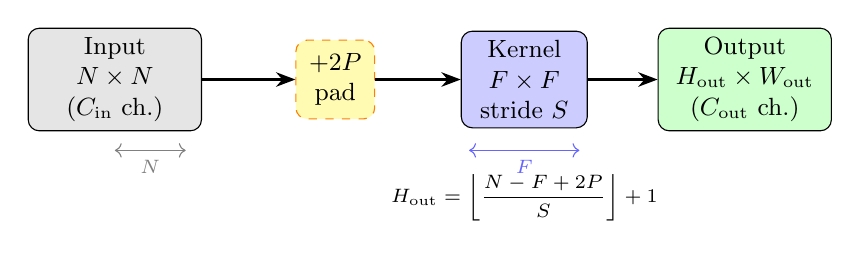
\begin{tikzpicture}[
  box/.style={draw, fill=#1, rounded corners=4pt, minimum height=1.0cm,
              font=\small, align=center},
  label/.style={font=\scriptsize, align=center},
  arrow/.style={-{Stealth[length=7pt]}, thick}
]

%% Input grid (5x5 shown as block)
\node[box=gray!20, minimum width=2.2cm] (inp) at (0,0)
  {Input\\$N \times N$\\$(\Cin$ ch.)};

%% Padding annotation
\node[box=yellow!30, minimum width=1.0cm, minimum height=1.0cm,
      dashed, draw=orange] (pad) at (2.8,0)
  {$+2P$\\pad};

%% Kernel
\node[box=blue!20, minimum width=1.6cm] (kern) at (5.2,0)
  {Kernel\\$F \times F$\\stride $S$};

%% Output
\node[box=green!20, minimum width=2.2cm] (out) at (8.0,0)
  {Output\\$H_{\mathrm{out}} \times W_{\mathrm{out}}$\\$(\Cout$ ch.)};

\draw[arrow] (inp.east) -- (pad.west);
\draw[arrow] (pad.east) -- (kern.west);
\draw[arrow] (kern.east) -- (out.west);

%% Formula below
\node[label] at (5.2,-1.5)
  {$H_{\mathrm{out}} = \left\lfloor\dfrac{N - F + 2P}{S}\right\rfloor + 1$};

%% Annotations
\draw[<->, gray, thin] (0,-0.9) -- node[below, font=\scriptsize]{$N$} (0.9,-0.9);
\draw[<->, blue!60, thin] (4.5,-0.9)
  -- node[below, font=\scriptsize]{$F$} (5.9,-0.9);

\end{tikzpicture}
\caption{Schematic of the convolution output size computation.
  Padding $P$ enlarges the effective input, the kernel of size $F$ slides
  across it with stride $S$, and the floor operation accounts for the
  integer number of complete strides.}
\label{fig:output_size}
\end{figure}

\begin{warningbox}
A common error is to forget the $+1$ term in \cref{eq:output_size}. This
term counts the initial filter placement at position 0 before any stride
steps are taken. Without it, the formula underestimates the output size by 1
in each spatial dimension. For a $5 \times 5$ input with a $3 \times 3$
filter and no padding: $\floor{(5-3)/1}+1 = 3$, not 2.
\end{warningbox}

% ════════════════════════════════════════════════════════════════════════════
\section{L2 Regularisation and Weight Decay}
\label{sec:l2reg}
% ════════════════════════════════════════════════════════════════════════════

\subsection{Motivation: Overfitting and Generalisation}

When a neural network has many more parameters than training samples, or
when training runs for many epochs, it can memorise the training data rather
than learning transferable features. This phenomenon---\emph{overfitting}---
manifests as low training loss but high validation/test loss.

Regularisation adds a penalty term to the loss that discourages excessively
large weights, biasing the optimiser toward solutions that generalise better.

\subsection{Mathematical Formulation}

\begin{definition}[L2 Regularised Loss]
\label{def:l2_loss}
The L2 regularised total loss is:
\begin{equation}
  \label{eq:l2_loss}
  \Ltotal = \Ldata + \lambda \sum_{i} w_i^2
\end{equation}
where $\Ldata$ is the task loss (cross-entropy, MSE, etc.),
$w_i$ are the learnable weight parameters (biases are typically excluded),
and $\lambda > 0$ is the regularisation strength.
\end{definition}

The penalty $\lambda \sum_i w_i^2$ penalises large-magnitude weights
quadratically, so the optimiser is incentivised to keep all weights small
unless forced large by the data loss.

\subsection{Gradient Update with L2 Penalty}

Taking the gradient of \cref{eq:l2_loss} with respect to a single weight
$w$:

\begin{align}
  \frac{\partial \Ltotal}{\partial w}
    &= \frac{\partial \Ldata}{\partial w} + 2\lambda w
  \label{eq:l2_grad}
\end{align}

The standard gradient descent update then becomes:

\begin{align}
  w &\leftarrow w - \eta \frac{\partial \Ltotal}{\partial w} \notag \\
    &= w - \eta \left(\frac{\partial \Ldata}{\partial w} + 2\lambda w\right)
       \notag \\
    &= w\bigl(1 - 2\eta\lambda\bigr)
       - \eta \frac{\partial \Ldata}{\partial w}
  \label{eq:weight_decay_update}
\end{align}

\begin{keyinsight}
\Cref{eq:weight_decay_update} reveals why L2 regularisation is also called
\textbf{weight decay}: the factor $(1 - 2\eta\lambda)$ \emph{decays} every
weight toward zero at each step, regardless of the gradient. The data
gradient then ``pushes back'' to maintain useful representations. The
balance between decay and push-back determines the effective magnitude of
learned weights.
\end{keyinsight}

\subsection{The Factor-of-Two Convention}

During the session, students raised the question of whether the gradient
update involves $2\lambda$ or $\lambda$. This depends on which convention
is used for the penalty:

\begin{align}
  \text{Convention A (standard):}\quad
    &\mathcal{L}_{\mathrm{reg}} = \lambda \sum_i w_i^2
    &&\Rightarrow\; \nabla_w \mathcal{L}_{\mathrm{reg}} = 2\lambda w
    \label{eq:conv_a} \\[4pt]
  \text{Convention B (divided by 2):}\quad
    &\mathcal{L}_{\mathrm{reg}} = \frac{\lambda}{2} \sum_i w_i^2
    &&\Rightarrow\; \nabla_w \mathcal{L}_{\mathrm{reg}} = \lambda w
    \label{eq:conv_b}
\end{align}

\noindent
The instructors confirmed that exam questions follow \textbf{Convention A}
unless the question explicitly provides a formula with $\tfrac{1}{2}$.
Students should read the question statement carefully and use whichever form
is given.

\begin{remark}
\label{rem:pytorch_convention}
PyTorch's \texttt{weight\_decay} parameter in SGD and Adam implements
\emph{weight decay} directly (multiplying weights by $(1-\eta\lambda_{\mathrm{wd}})$
per step), which corresponds to Convention B at the gradient level. For most
practical purposes the distinction does not matter because $\lambda$ is
tuned empirically. However, for numeric exam questions, one must use the
exact formula provided.
\end{remark}

\subsection{PyTorch Implementation}

L2 regularisation is activated by passing a non-zero \texttt{weight\_decay}
argument to any PyTorch optimiser:

\begin{verbatim}
import torch.optim as optim

# Adam with L2 regularisation (weight_decay acts as lambda)
optimizer = optim.Adam(model.parameters(),
                       lr=1e-3,
                       weight_decay=1e-4)   # lambda = 0.0001

# SGD with weight decay and momentum
optimizer = optim.SGD(model.parameters(),
                      lr=1e-1,
                      weight_decay=1e-4,
                      momentum=0.9)
\end{verbatim}

\noindent
\textbf{Default:} \texttt{weight\_decay=0}, meaning no regularisation is
applied unless explicitly set.

\subsection{Effect on the Loss Surface}

Adding the L2 term reshapes the optimisation landscape. The effective loss
becomes a sum of the data loss and a bowl-shaped quadratic. This has three
practical consequences:

\begin{enumerate}[label=\textbf{(\roman*)}]
  \item \textbf{Unique minimum}: Even if $\Ldata$ has flat directions (e.g.,
        under-determined systems), the L2 term creates a unique minimum at
        $\mathbf{w} = \mathbf{0}$ in the absence of data.
  \item \textbf{Smaller weights}: The optimal weights are pulled toward zero
        relative to the unregularised solution.
  \item \textbf{Smoother decision boundaries}: Smaller weights in
        classification networks imply flatter activation surfaces, reducing
        the risk of sharp spurious boundaries that do not generalise.
\end{enumerate}

\begin{table}[ht]
  \centering
  \caption{Effect of \texttt{weight\_decay} (L2 regularisation strength) on
    model behaviour. Typical experimental observations.}
  \label{tab:l2_effect}
  \begin{tabularx}{\linewidth}{@{}lXX@{}}
    \toprule
    \texttt{weight\_decay} & Effect on training & Effect on generalisation \\
    \midrule
    $0$ (default)
      & Weights grow freely; fast convergence on training set
      & Risk of overfitting; poor test performance if data is scarce \\
    $10^{-4}$ (light)
      & Slight weight shrinkage; negligible training loss impact
      & Small generalisation improvement; common default choice \\
    $10^{-3}$ (moderate)
      & Noticeable weight shrinkage; may slow convergence
      & Better generalisation; can under-fit if combined with small model \\
    $10^{-2}$ (strong)
      & Heavy weight shrinkage; training loss visibly higher
      & Strong bias toward zero weights; often too aggressive \\
    \bottomrule
  \end{tabularx}
\end{table}

% ════════════════════════════════════════════════════════════════════════════
\section{Comparative Analysis and Design Decisions}
\label{sec:comparison}
% ════════════════════════════════════════════════════════════════════════════

\subsection{Parameter Efficiency: Conv vs FC vs Depthwise Conv}

To place Session 15's parameter-counting exercise in a broader context,
\cref{tab:arch_comparison} compares several layer types for the
same $\Cin = 128$, $\Cout = 64$ transformation.

\begin{table}[ht]
  \centering
  \caption{Parameter counts for different layer types with
    $\Cin=128$, $\Cout=64$, $F=3$.}
  \label{tab:arch_comparison}
  \begin{tabularx}{\linewidth}{@{}Xrrl@{}}
    \toprule
    Layer type & Weight params & Bias & Total \\
    \midrule
    \texttt{Conv2d(128,64,3)} (standard)
      & 73,728 & 64 & 73,792 \\
    \texttt{Conv2d(128,64,1)} ($1\times1$ conv)
      & 8,192  & 64 & 8,256 \\
    Depthwise \texttt{Conv2d(128,128,3)} + pointwise
      & $9\times128 + 128\times64 = 1152+8192$
      & $128+64$ & 9,536 \\
    \texttt{Linear(128,64)} (no spatial)
      & 8,192 & 64 & 8,256 \\
    \texttt{Linear(7$\times$7$\times$128, 64)} (flattened)
      & 401,408 & 64 & 401,472 \\
    \bottomrule
  \end{tabularx}
\end{table}

\noindent
The depthwise-separable factorisation used in MobileNet achieves roughly the
same representation with $\sim$8$\times$ fewer parameters than standard
\texttt{Conv2d}.

\subsection{Regularisation Strategies: L2 vs Dropout vs Batch Norm}

L2 regularisation is one of several complementary strategies available in
deep learning. \Cref{tab:reg_comparison} provides a side-by-side comparison.

\begin{table}[ht]
  \centering
  \caption{Comparison of regularisation strategies.}
  \label{tab:reg_comparison}
  \begin{tabularx}{\linewidth}{@{}lXXX@{}}
    \toprule
    Technique & Mechanism & Hyperparameter & Typical use \\
    \midrule
    L2 (weight decay)
      & Penalises large weights; shrinks weights toward zero
      & \texttt{weight\_decay} $\lambda$
      & Almost always used; \texttt{1e-4} default \\
    L1 regularisation
      & Penalises absolute weight magnitude; encourages sparsity
      & Regularisation coefficient
      & Sparse models, feature selection \\
    Dropout
      & Randomly zeros activations during training
      & Drop probability $p$
      & FC layers; \texttt{p=0.5} classic \\
    Batch Normalisation
      & Normalises layer inputs; implicit regularisation
      & Momentum, $\epsilon$
      & Between conv and activation \\
    Data Augmentation
      & Expands effective training set via transforms
      & Augmentation policy
      & Image tasks; near-zero cost \\
    Early Stopping
      & Halts training when validation loss increases
      & Patience epochs
      & Universal safety net \\
    \bottomrule
  \end{tabularx}
\end{table}

\subsection{Padding Regime Tradeoffs}

\begin{keyinsight}
The choice of padding regime affects both the output spatial dimension and
the receptive field coverage at the feature map borders:
\begin{itemize}[noitemsep]
  \item \textbf{Valid padding ($P=0$)}: Spatial dimensions shrink with depth;
        border pixels appear in fewer filter applications. Used in LeNet-5
        and early CNNs.
  \item \textbf{Same padding ($P=(F{-}1)/2$)}: Spatial dimensions preserved;
        all positions receive equal filter coverage. Used in VGG, ResNet,
        and modern architectures.
  \item \textbf{Strided convolution ($S=2$, $P=0$)}: Spatial downsampling
        without pooling; the stride itself performs subsampling. Preferred in
        modern efficient architectures (e.g., ResNet stem, DCGAN generator).
\end{itemize}
\end{keyinsight}

% ════════════════════════════════════════════════════════════════════════════
\section{Unified TikZ Architecture Diagram}
\label{sec:architecture}
% ════════════════════════════════════════════════════════════════════════════

\Cref{fig:cnn_pipeline} shows the full computation pipeline for a single
convolutional block, annotating where the output size formula
(\cref{eq:output_size}) and parameter count formula (\cref{eq:param_formula})
apply.

\begin{figure}[ht]
\centering
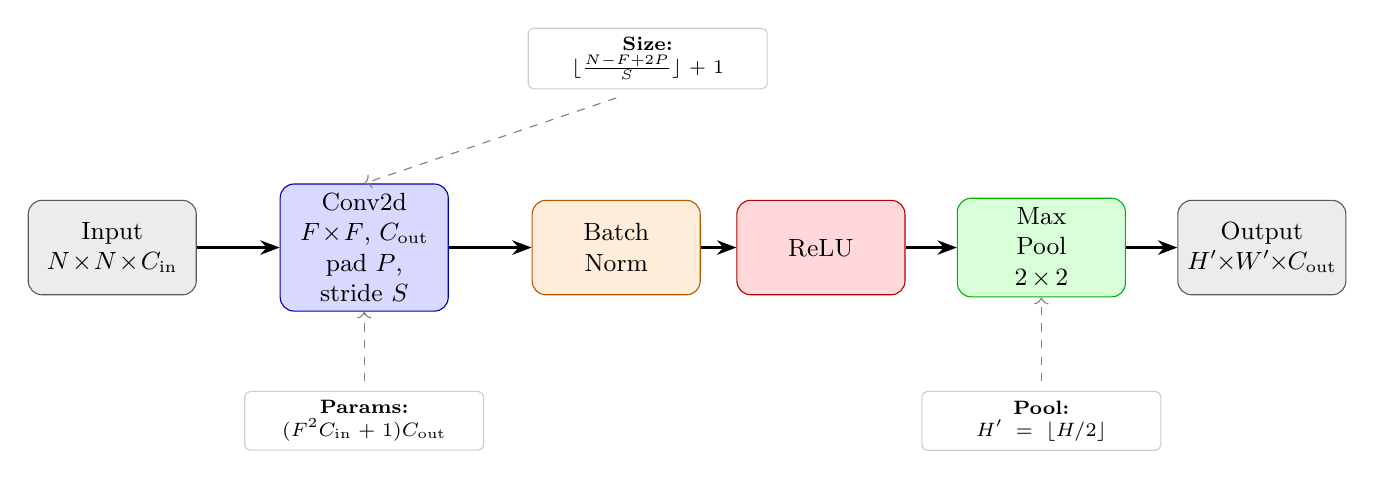
\begin{tikzpicture}[
  blk/.style={draw=#1!70!black, fill=#1!15, rounded corners=5pt,
              minimum width=2.0cm, minimum height=1.2cm,
              font=\small, align=center, text width=1.9cm},
  ann/.style={font=\scriptsize, draw=gray!40, fill=white,
              rounded corners=2pt, align=center, text width=2.8cm},
  arrow/.style={-{Stealth[length=7pt]}, thick, #1},
  every node/.style={align=center}
]

%% Nodes left to right
\node[blk=gray]   (inp)  at (0,   0) {Input\\$N\!\times\!N\!\times\!\Cin$};
\node[blk=blue]   (conv) at (3.2, 0) {Conv2d\\$F\!\times\!F$, $\Cout$\\pad $P$, stride $S$};
\node[blk=orange] (bn)   at (6.4, 0) {Batch\\Norm};
\node[blk=red]    (act)  at (9.0, 0) {ReLU};
\node[blk=green]  (pool) at (11.8,0) {Max\\Pool\\$2\!\times\!2$};
\node[blk=gray]   (out)  at (14.6,0) {Output\\$H'\!\times\!W'\!\times\!\Cout$};

%% Arrows
\draw[arrow={}] (inp.east)  -- (conv.west);
\draw[arrow={}] (conv.east) -- (bn.west);
\draw[arrow={}] (bn.east)   -- (act.west);
\draw[arrow={}] (act.east)  -- (pool.west);
\draw[arrow={}] (pool.east) -- (out.west);

%% Annotation: parameter count
\node[ann] at (3.2, -2.2)
  {\textbf{Params:}\\$(F^2\Cin+1)\Cout$};
\draw[->, dashed, gray] (3.2,-1.7) -- (conv.south);

%% Annotation: output size
\node[ann] at (6.8, 2.4)
  {\textbf{Size:}\\$\lfloor\frac{N-F+2P}{S}\rfloor+1$};
\draw[->, dashed, gray] (6.4,1.9) -- (conv.north);

%% Annotation: pool halves
\node[ann] at (11.8,-2.2)
  {\textbf{Pool:}\\$H' = \lfloor H/2\rfloor$};
\draw[->, dashed, gray] (11.8,-1.7) -- (pool.south);

\end{tikzpicture}
\caption{Typical CNN convolutional block pipeline. The parameter count
  formula applies at the \texttt{Conv2d} step; the output size formula
  applies at both \texttt{Conv2d} and \texttt{MaxPool2d}. BatchNorm and
  ReLU do not change spatial dimensions and have no (or negligible) learnable
  parameters.}
\label{fig:cnn_pipeline}
\end{figure}

% ════════════════════════════════════════════════════════════════════════════
\section{Session Q\&A: Detailed Walkthroughs}
\label{sec:qa}
% ════════════════════════════════════════════════════════════════════════════

This section provides extended solutions to the questions raised during
Session 15.

\subsection{Q1: Counting Parameters with Bias}

\textbf{Question (paraphrased from session):} \\
\textit{A convolution layer has 64 filters, kernel size $3 \times 3$, and
128 input channels. Should we include bias? How many parameters total?}

\textbf{Answer:} \\
Yes, bias is included by default in PyTorch (\texttt{bias=True}). Using
\cref{eq:param_formula}:

\begin{align*}
  P &= (F^2 \cdot \Cin + 1) \cdot \Cout \\
    &= (9 \cdot 128 + 1) \cdot 64 \\
    &= 1153 \cdot 64 \\
    &= \mathbf{73{,}792}
\end{align*}

\textbf{Choice of correct answer:} If the multiple-choice options include
both $73{,}728$ (no bias) and $73{,}792$ (with bias), and the question does
not specify \texttt{bias=False}, select $73{,}792$.

\subsection{Q2: L2 Penalty Contribution --- Theory vs PyTorch}

\textbf{Question (paraphrased from session):} \\
\textit{Given weight decay $\lambda = 10^{-4}$ and weights
$\mathbf{w} = [w_1, w_2, \ldots]$, what is the L2 penalty contribution to
the loss? There seem to be two formulas (theoretical and PyTorch). Which do
we use?}

\textbf{Answer:} \\
For exam purposes, use the \textbf{theoretical formula}:
\begin{equation}
  \mathcal{L}_{\mathrm{L2}} = \lambda \sum_i w_i^2
  \label{eq:l2_penalty_qa}
\end{equation}

If the exam question provides a formula that includes $\tfrac{1}{2}$:
\[
  \mathcal{L}_{\mathrm{L2}} = \frac{\lambda}{2} \sum_i w_i^2
\]
then use \emph{that} formula instead and do \emph{not} include the factor
of 2 in the gradient. The key signal is: \textbf{use whichever formula is
given in the question}.

\textbf{Numerical example:} With $\lambda = 10^{-4}$ and weights
$\mathbf{w} = [0.5, -0.3, 0.8]$:
\begin{align*}
  \sum_i w_i^2 &= 0.25 + 0.09 + 0.64 = 0.98 \\
  \mathcal{L}_{\mathrm{L2}} &= 10^{-4} \times 0.98 = 9.8 \times 10^{-5}
\end{align*}

\subsection{Q3: Output Size for Standard Layers}

\textbf{Question:} \\
\textit{What is the output size after \texttt{Conv2d(128, 64, kernel\_size=3,
stride=1, padding=0)} applied to a $7 \times 7$ feature map?}

\textbf{Answer:} Using \cref{eq:output_size} with $N=7$, $F=3$, $P=0$,
$S=1$:
\[
  H_{\mathrm{out}} = \floor{\frac{7 - 3 + 0}{1}} + 1 = 4 + 1 = \mathbf{5}
\]
Output: $5 \times 5 \times 64$.

% ════════════════════════════════════════════════════════════════════════════
\section{Transition to Recurrent Neural Networks}
\label{sec:rnn_preview}
% ════════════════════════════════════════════════════════════════════════════

Session 15 marks the end of the CNN module and the beginning of the
transition to \textbf{Recurrent Neural Networks} (RNNs), covered by the
\texttt{08\_PyTorchDL\_RNN} deck. This section briefly previews the
conceptual shift.

\subsection{Limitations of CNNs for Sequential Data}

CNNs operate on fixed-size inputs with no inherent notion of \emph{temporal
order}. When the input is a sequence (text, speech, time series), CNNs can
capture local patterns within a window via 1D convolutions, but they
\begin{itemize}[noitemsep]
  \item Cannot maintain \emph{state} across time steps,
  \item Require a fixed receptive field (context window), and
  \item Do not model variable-length dependencies.
\end{itemize}

\subsection{The RNN Paradigm}

RNNs address these limitations by introducing a \emph{hidden state}
$\mathbf{h}_t$ that is updated at each time step $t$:

\begin{equation}
  \mathbf{h}_t = \tanh\!\left(W_{hh}\,\mathbf{h}_{t-1}
                             + W_{xh}\,\mathbf{x}_t + \mathbf{b}\right)
  \label{eq:rnn_cell}
\end{equation}

where $\mathbf{x}_t$ is the input at step $t$, and
$W_{hh}$, $W_{xh}$, $\mathbf{b}$ are shared parameters across all time
steps (analogous to weight sharing in CNNs).

\begin{keyinsight}
The same weight matrices $(W_{hh}, W_{xh})$ are applied at every time step,
just as the same filter weights are applied at every spatial location in a
CNN. This is the RNN analogue of \textbf{weight sharing across time}.
\end{keyinsight}

\begin{table}[ht]
  \centering
  \caption{CNN vs RNN conceptual comparison.}
  \label{tab:cnn_vs_rnn}
  \begin{tabularx}{\linewidth}{@{}lXX@{}}
    \toprule
    Concept & CNN (spatial) & RNN (temporal) \\
    \midrule
    Input structure   & Grid ($H \times W \times C$)
                      & Sequence ($T \times d$) \\
    Shared parameters & Filter weights across spatial locations
                      & Weight matrices across time steps \\
    State             & Feature maps (static)
                      & Hidden state $\mathbf{h}_t$ (evolves) \\
    Inductive bias    & Local spatial patterns
                      & Temporal dependencies \\
    Depth             & Number of stacked conv layers
                      & Sequence length (unrolled depth) \\
    Gradient issue    & Vanishing gradients (deep nets)
                      & Vanishing/exploding gradients (long sequences) \\
    \bottomrule
  \end{tabularx}
\end{table}

\noindent
The RNN module will cover vanilla RNNs, Long Short-Term Memory (LSTM) cells,
and Gated Recurrent Units (GRUs), building on the same parameter-counting
and regularisation foundations established in the CNN module.

% ════════════════════════════════════════════════════════════════════════════
\section{Summary and Conclusions}
\label{sec:conclusion}
% ════════════════════════════════════════════════════════════════════════════

Session 15 served as a focused consolidation session before transitioning
to the RNN module. The three core topics revisited and clarified were:

\begin{enumerate}[label=\textbf{(\arabic*)}, leftmargin=2em]

  \item \textbf{Convolutional layer parameter counting}
    (\cref{sec:param_count}): The formula
    $(F^2 \cdot \Cin + 1) \cdot \Cout$ gives the exact number of trainable
    parameters in a \texttt{Conv2d} layer, \emph{independent of the input
    spatial size}. For the exam example of 64 filters, $3\times3$ kernels,
    128 input channels, the answer is \textbf{73,792} with bias (73,728
    without). This is $\sim$$5.4\times$ fewer than the equivalent fully-connected
    layer ($\sim$401,472), illustrating the efficiency of weight sharing.

  \item \textbf{Convolution output size formula}
    (\cref{sec:output_size}): The general formula is
    $\floor{(N - F + 2P)/S} + 1$. The three key configurations are
    \emph{valid} ($P=0$), \emph{same} ($P=(F{-}1)/2$, preserves size for
    odd $F$), and \emph{strided} ($S=2$, halves spatial dimensions). The
    $+1$ term is frequently omitted in error and must always be included.

  \item \textbf{L2 regularisation and weight decay}
    (\cref{sec:l2reg}): The regularised loss
    $\Ldata + \lambda\sum_i w_i^2$ penalises large weights quadratically.
    The resulting gradient update $(1 - 2\eta\lambda)w -
    \eta\nabla_w\Ldata$ is called weight decay because it shrinks weights
    at every step. In PyTorch, this is controlled by the
    \texttt{weight\_decay} argument to any optimiser. For exam calculations,
    use the formula provided in the question---with or without the factor of
    $\tfrac{1}{2}$ depending on what is stated.

\end{enumerate}

\medskip

\noindent
\textbf{Preview of Session 16 (RNNs):}
The next session introduces Recurrent Neural Networks using the
\texttt{08\_PyTorchDL\_RNN} slide deck. The same principles of weight
sharing, parameter counting, and regularisation carry over, now applied
to sequences rather than spatial feature maps.

\begin{keyinsight}
Three formulae to commit to memory from Session 15:
\begin{align*}
  \text{Conv params:}\quad
    & P = (F^2 \cdot \Cin + 1) \cdot \Cout \\
  \text{Output size:}\quad
    & H_{\mathrm{out}} = \floor{\frac{N - F + 2P}{S}} + 1 \\
  \text{L2 loss:}\quad
    & \Ltotal = \Ldata + \lambda\sum_i w_i^2
\end{align*}
\end{keyinsight}

% ════════════════════════════════════════════════════════════════════════════
%  APPENDIX
% ════════════════════════════════════════════════════════════════════════════
\appendix

\section{Quick-Reference Formula Sheet}
\label{app:formulas}

\subsection*{Convolutional Layer --- Parameter Count}
\[
  P_{\mathrm{conv}} = (F \times F \times \Cin + b) \times \Cout,
  \quad b = \begin{cases}1 & \text{bias=True (default)}\\0 & \text{bias=False}\end{cases}
\]

\subsection*{Convolution Output Size}
\[
  H_{\mathrm{out}} = \floor{\frac{N - F + 2P}{S}} + 1
\]

\textbf{Special cases:}
\begin{itemize}[noitemsep]
  \item Same padding: $P = (F-1)/2$, $S=1$ $\Rightarrow$ $H_{\mathrm{out}} = N$
  \item Valid padding: $P=0$, $S=1$ $\Rightarrow$ $H_{\mathrm{out}} = N - F + 1$
  \item Stride-2 downsampling: $P=0$, $S=2$ $\Rightarrow$
        $H_{\mathrm{out}} = \floor{(N-F)/2} + 1$
\end{itemize}

\subsection*{L2 Regularised Loss and Gradient}
\begin{align*}
  \Ltotal &= \Ldata + \lambda \sum_i w_i^2 \\
  \frac{\partial \Ltotal}{\partial w} &= \frac{\partial \Ldata}{\partial w} + 2\lambda w \\
  w &\leftarrow w\,(1 - 2\eta\lambda)
    - \eta\,\frac{\partial \Ldata}{\partial w}
\end{align*}

\subsection*{Typical Hyperparameter Ranges}
\begin{center}
\begin{tabular}{@{}lll@{}}
  \toprule
  Hyperparameter & Symbol & Typical range \\
  \midrule
  Learning rate (SGD)      & $\eta$ & $0.1$, $0.01$, $0.001$ \\
  Learning rate (Adam)     & $\eta$ & $10^{-3}$ \\
  Weight decay (L2)        & $\lambda$ & $10^{-4}$--$10^{-2}$ \\
  Momentum                 & $\mu$ & $0.9$ \\
  Dropout probability      & $p$ & $0.3$--$0.5$ \\
  \bottomrule
\end{tabular}
\end{center}

\section{Session Metadata}
\label{app:metadata}

\begin{center}
\begin{tabular}{@{}ll@{}}
  \toprule
  Field & Value \\
  \midrule
  Session       & 15 \\
  Format        & Interactive Q\&A / doubt-clearing \\
  Duration      & $\approx$ 1 hour 10 minutes \\
  Instructors   & Prof.\ S.~R.~M.\ Prasanna, Dr.\ Sunil Saumya \\
  Institution   & IIIT Dharwad \\
  Slide deck    & \texttt{08\_PyTorchDL\_RNN} \\
  Video URL     & \url{https://vimeo.com/1153110691} \\
  Preceding topic & CNNs with PyTorch (Sessions 10--14) \\
  Following topic & Recurrent Neural Networks (Session 16+) \\
  Topics covered  & Conv param counting, output size, L2 regularisation \\
  \bottomrule
\end{tabular}
\end{center}

\end{document}
